\section{Inbetriebnahme von Keysight Advanced Design System (ADS)}
\subsection{Installation von ADS}
Die Software \ac{ADS} dient zur Simulation von Schaltungen verschiedener Komplexitätsgrade. 
In diesem Versuch wird die Software verwendet, um eine Hochfrequenzschaltung zu simulieren und zu analysieren. 
Die Software bietet eine Vielzahl von Funktionen, darunter die Möglichkeit, Schaltungen zu entwerfen, S-Parameter zu simulieren und verschiedene Analysewerkzeuge zu verwenden.

\subsection{Erstellen eines neuen Projekts}
Die Software ist auf den Rechnern im Labor bereits installiert gewesen. 
Nach dem Start der Software wird ein neues Projekt aus den bereits zur Verfügung stehenden Workspaces erstellt. 
Diese sind auf der ILIAS-Seite des Praktikums in dem Dateiarchiv \texttt{TransmitterAmpDesign 2024.zip} hinterlegt. 
Die Datei wird entpackt und in der Software geöffnet. Außerdem werden die benötigten Bibliotheken aus dem Dateiarchiv \texttt{Infineon-RFTransistor-Keysight ADS Design Kit-SM-v02 10-EN.zip} geladen, diese stehen ebenfalls auf der ILIAS-Seite zur Verfügung.
\subsection{Vertrautmachen mit der Benutzeroberfläche}
Schließlich werden die Tutorials 1 und 2 von \ac{ADS} durchgearbeitet, um sich mit der Benutzeroberfläche und den grundlegenden Funktionen der Software vertraut zu machen.
Am Anfang der Schaltungsanalyse wird das Schema \texttt{TX\_Amp\_Bias.dds} geöffnet. Diese ist in der Abbildung \ref{fig:TX_BIAS} zu sehen.

\begin{figure}[h]
    \centering
    \includegraphics[width=0.7\textwidth]{Pictures/TX_BIAS.png}
    \caption{Schaltbild der Schaltung \texttt{TX\_Amp\_Bias.dds} in \ac{ADS}.}
    \label{fig:TX_BIAS}
\end{figure}

\section{Analyse des Datenblattes zu Transistor BFR181W}
Um die Schaltung zu simulieren, wird der Transistor BFR181W verwendet. Um die genauen Parameter des Transistors zu kennen, wird das Datenblatt des Transistors analysiert.
Dieses steht auch auf der ILIAS-Seite des Praktikums zur Verfügung.

Die Tabelle \enquote{Maximum Ratings at $T_\mathrm{A}=25\,^\circ\mathrm{C}$, unless otherwise specified} unten links auf Seite 1 des Dokuments zeigt, dass der maximal zulässige Kollektorstrom $I_{C,\mathrm{max}}$ 20\,mA beträgt.
\section{DC-Simulation}
Im folgendem wird eine DC-Simulation der später aufzubauenden Schaltung durchgeführt. 
Außerdem werden die Arbeitspunkte optimal durch die Anpassung der Widerstandswerte eingestellt.
Die DC-Simulation wird in \ac{ADS} durchgeführt, um die DC-Pegel der Schaltung zu überprüfen.
\clearpage
\subsection{Dimensionierung des Kollektorwiderstandes}
Folgende Spannungswerte werden angenommen:
\begin{itemize}
    \item $U_{CC} = 4.8\,\mathrm{V}$
    \item $U_{BE} = 0.77\,\mathrm{V}$
\end{itemize}

Zuerst wird der Kollektorwiderstand $R_5$ passend gewählt, sodass der Kollektorstrom $I_C$ auf $75\,\%$ des maximal zulässigen Kollektorstroms $I_{C,\mathrm{max}}$ gesetzt wird. 
Dies geschieht, indem der Widerstandswert $R_5$ so gewählt wird, dass der Kollektorstrom $I_C$ 15\,mA beträgt.
Der Widerstandswert $R_5$ wird mit folgender Formel berechnet:
\begin{equation}
    R_5 = \frac{U_{CC} - U_{CE}}{I_C} = \frac{4.8\,\mathrm{V}}{15\,\mathrm{mA}} = 320\,\Omega
\end{equation}

Bei der Verwendung der E12-Reihe wird eine Faustregel verwendet, nach der man die Widerstandswerte auf die nächstgelegene E12-Reihe aufrundet. 
Somit beträgt der errechnete Widerstandswert von $R_5$ 330\,\(\Omega\). Dadurch wird der in den Kollektor eingehende Strom beschränkt, was eine Überlastung des Transistors im Dauerbetrieb vorbeugt. Bei der Wahl eines niedrigeren Widerstandswertes würde der Kollektorstrom $I_C$ den maximalen Kollektorstrom $I_{C,\mathrm{max}}$ überschreiten, was zu einer Überlastung des Transistors führen würde.

Dieses Ergebnis lässt sich anhand der Simulation in \ac{ADS} verifizieren. Es wird ein Sweep des Kollektorwiderstandes $R_5$ in der Spanne von 100\,\(\Omega\) bis 4,7\,k\(\Omega\) durchgeführt.
Es ergibt sich der folgende Verlauf des Kollektorstroms $I_C$ in Abhängigkeit des Kollektorwiderstandes $R_5$:
\begin{figure}[H] % Fix: [H] erzwingt die Platzierung genau hier
    \centering
    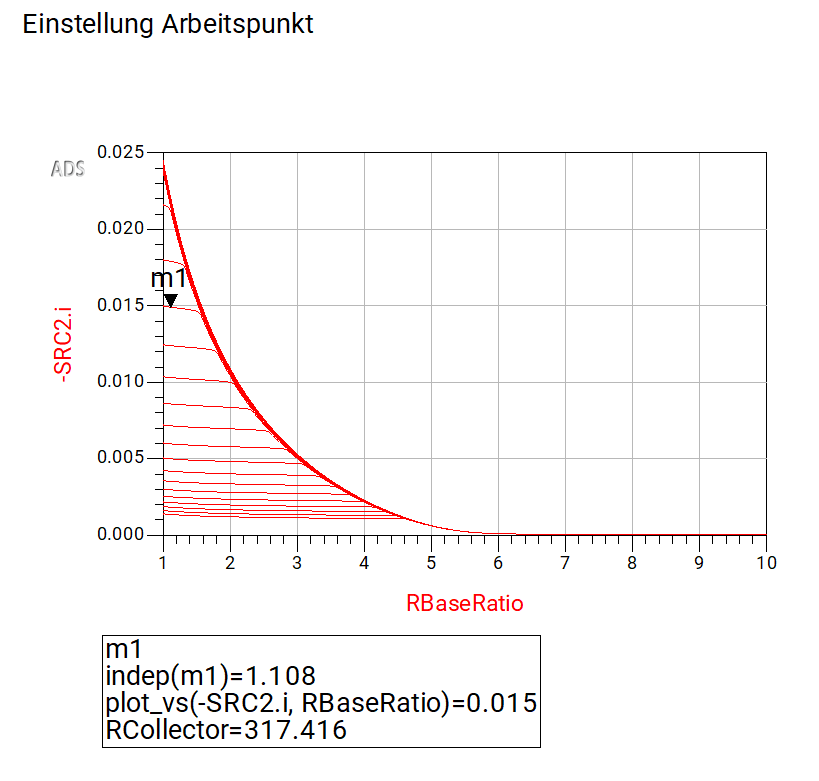
\includegraphics[width=0.7\textwidth]{Pictures/RCollector.png}
    \caption{Verlauf des Kollektorstroms $I_C$ in Abhängigkeit des Kollektorwiderstandes $R_5$.}
    \label{fig:RCollector}
\end{figure}

Aus der Abbildung \ref{fig:RCollector} ist zu erkennen, dass der Kollektorstrom $I_C$ mit steigendem Kollektorwiderstand $R_5$ abnimmt. Mit dem Marker m1 wird außerdem
gezeigt, dass der Kollektorstrom $I_C$ bei einem Widerstandswert von 317,416\,\(\Omega\) einen Wert von 15\,mA erreicht. Es wird der nächstgrößere Widerstandswert der E12-Reihe gewählt, also 330\,\(\Omega\).
Die Ergebnisse der Rechnung wurden also somit bestätigt.

\subsection{Dimensionierung des Basis-Spannungsteilers}

Um einen Arbeitspunkt mit $I_C \approx 10\,\mathrm{mA}$ zu erreichen, wird der Basis-Spannungsteiler dimensioniert. Die Basis-Emitter-Spannung beträgt $U_{BE} \approx 0{,}7\,\mathrm{V}$. Der Emitterwiderstand wird hier vernachlässigt.

Der Basisstrom berechnet sich zu:
\begin{equation}
    I_B = \frac{I_C}{\beta}
\end{equation}
Für einen typischen Verstärkungsfaktor $\beta = 100$ ergibt sich:
\begin{equation}
    I_B = \frac{10\,\mathrm{mA}}{100} = 0{,}1\,\mathrm{mA} = 100\,\mu\mathrm{A}
\end{equation}

Der Querstrom des Spannungsteilers $I_Q$ sollte mindestens das 10-fache des Basisstroms betragen:
\begin{equation}
    I_Q = 10 \cdot I_B = 1{,}0\,\mathrm{mA}
\end{equation}

Die Basisspannung $U_B$ ergibt sich zu:
\begin{equation}
    U_B = U_{BE} + U_E \approx 0{,}77\,\mathrm{V}
\end{equation}

Angenommen, die Betriebsspannung ist $U_{CC} = 4{,}8\,\mathrm{V}$, ergibt sich für die Widerstände $R_4$ (oben) und $R_3$ (unten):
\begin{align}
    R_3 &= \frac{U_B}{I_Q} = \frac{0{,}77\,\mathrm{V}}{1{,}0\,\mathrm{mA}} = 0{,}77\,\mathrm{k}\Omega \\
    R_4 &= \frac{U_{CC} - U_B}{I_Q} = \frac{4{,}8\,\mathrm{V} - 0{,}77\,\mathrm{V}}{1{,}0\,\mathrm{mA}} = 4{,}03\,\mathrm{k}\Omega
\end{align}

Nach der Berechnung ergibt sich für $R_3$ ein Wert von $0{,}77\,\mathrm{k}\Omega$. In der praktischen Simulation mit ADS zeigte sich jedoch, dass mit diesem Wert ein negatives Gain bei der S-Parameter-Simulation auftritt. Daher wird $R_3$ nach der E12-Reihe auf $1{,}0\,\mathrm{k}\Omega$ erhöht, um einen stabilen Arbeitspunkt und ein positives Verstärkungsverhalten zu gewährleisten.

Mit der E12-Reihe werden gewählt:
\begin{align*}
    R_3 &= 1{,}0\,\mathrm{k}\Omega \\
    R_4 &= 4{,}7\,\mathrm{k}\Omega
\end{align*}

Damit ist der Spannungsteiler dimensioniert, sodass im Arbeitspunkt ein Kollektorstrom von ca. $10\,\mathrm{mA}$ zu erwarten ist und die Simulation ein positives Gain liefert.
\section{S-Parameter-Simulation}
Schließlich wird die S-Parameter-Simulation durchgeführt. Diese ist wichtig, um einen angemessenen Gain bei der Übertragung zu gewährleisten.
Die S-Parameter-Simulation wird in \ac{ADS} nach folgenden Schritten durchgeführt:
\begin{enumerate}
    \item Im ADS-Model wird die Kommentierung des S-Parameter-Controllers aufgehoben, also die S-Parameter-Einstellung wird aktiviert.
    \item Da jetzt die DC-Simulation überflüssig ist, wird diese deaktiviert.
    \item Vor der Simulation wird die Schrittweite des S-Parameter-Controllers auf 250 MHz gesetzt, sodass man die Qualität des Frequenz-Sweeps verbessert.
    
\includegraphics[height=0.7cm]{Pictures/simulate.png}
    \item Nach der Simulation wird das Ergebnis in einem neuen Fenster angezeigt. Es ergibt sich der folgende Verlauf des Gains für verschiedene Frequenzen:
    
    \begin{figure}[h]
            \centering
            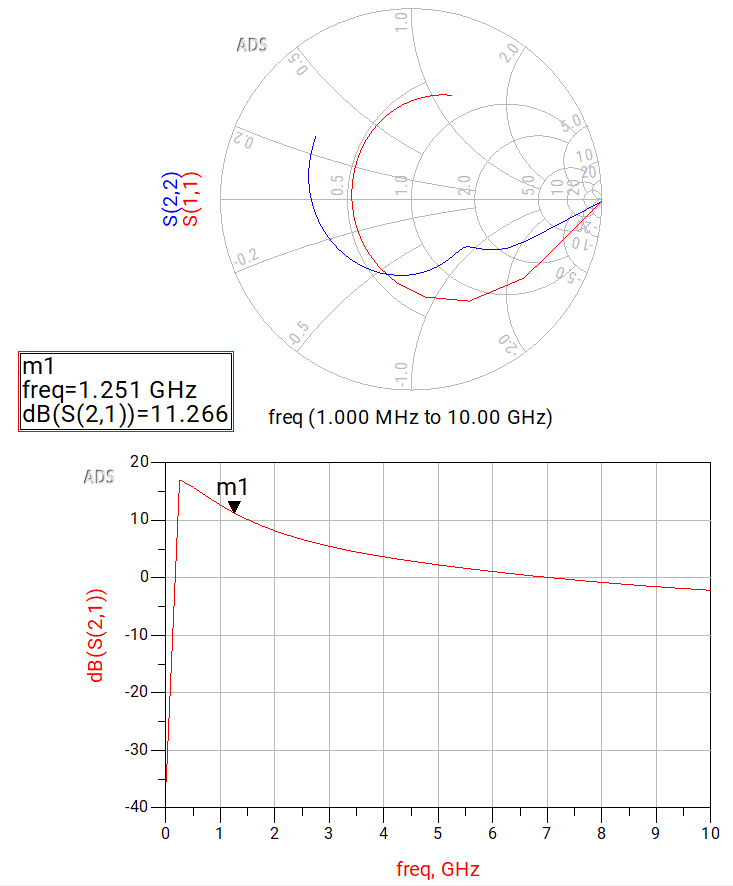
\includegraphics[width=0.7\textwidth]{Pictures/SParameter.png}
            \caption{Ergebnisse der S-Parameter-Simulation.}
            \label{fig:SParameter}
        \end{figure}
    
    Hier wählt man die Schaltfläche \enquote{Insert A New Marker} aus 
\includegraphics[height=0.5cm]{Pictures/marker.png}.
    Wir setzen den Marker auf den Punkt unserer Arbeitsfrequenz, also bei 1{,}25 GHz (s. Abbildung \ref{fig:SParameter}). Der Marker m1 zeigt eine \textbf{Verstärkung (Gain) von 11,266 dB} an.
\end{enumerate}


\clearpage
% Erklärung zu [h] und [H]:
%
% [h] ist ein "placement specifier" für Gleitobjekte (z.B. figure, table) und bedeutet "here" – also möglichst an der aktuellen Stelle im Text.
% LaTeX kann das Objekt aber trotzdem verschieben, wenn es an dieser Stelle nicht passt.
%
% [H] (nur mit \usepackage{float}) erzwingt die Platzierung GENAU an der Stelle im Quelltext, ohne Ausweichmöglichkeiten.
